\documentclass[a4paper]{article}

%% Page Size and Margins
\usepackage[a4paper,top=3cm,bottom=2cm,left=2cm,right=2cm,marginparwidth=1.75cm]{geometry}

%% Useful packages
\usepackage{graphicx}
\usepackage{fancyhdr}
\usepackage{hyperref}

%%\usepackage{amsmath}
%%\usepackage[colorinlistoftodos]{todonotes}
%%\usepackage[colorlinks=true, allcolors=blue]{hyperref}
%%\usepackage{caption}
%%\usepackage{subcaption}
%%\usepackage{sectsty}
%%\usepackage{apacite}
%%\usepackage{float}
%%\usepackage{titling} 
%%\usepackage{blindtext}
%%\usepackage[square,sort,comma,numbers]{natbib}
%%\usepackage[colorinlistoftodos]{todonotes}
%%\usepackage{xcolor}
%%\definecolor{darkgreen}{rgb}{0.0, 0.4, 0.0}

%% Document Begin
\begin{document}

%% titlepage
\begin{titlepage}
\vspace*{100px}
\newcommand{\HRule}{\rule{\linewidth}{0.5mm}} 	
\center 
 
% Fisrt row
{ \huge \bfseries Aurora-Remote}
\vspace*{50px}

% Program info
\HRule \\[0.8cm]

\textsc{\normalsize \emph {Ericsson C50 Aurora / Niros TRX3001 - Remote}}\\[0.8cm]

\HRule \\[1cm]

%%Picture
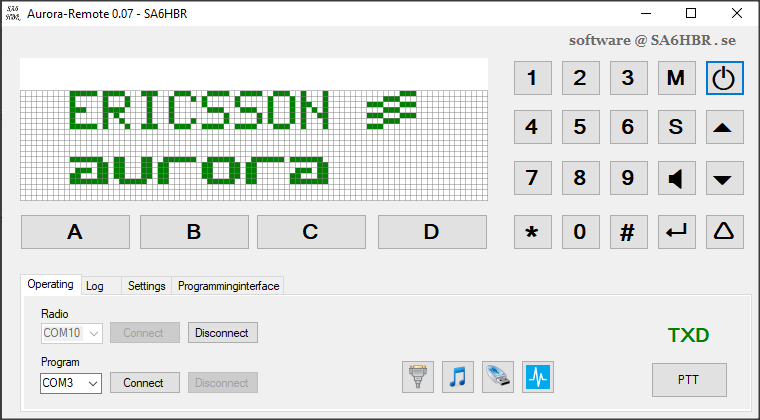
\includegraphics[width=0.6\textwidth]{../image/AuroraRemote.png}\\[3cm] 

{\large \today}\\[2cm]
\textsc{ \huge \bfseries SA6HBR}\\[1cm]

\vfill 
\end{titlepage}

\pagestyle{fancy}
\fancyhf{}
\lhead{\today}
\rhead{SA6HBR}

%%\lhead{Guides and tutorials}
\cfoot{ \thepage}

%% Section English
%%\section*{English}

%%Simple program for Remoteing serial communication
%%\newpage

%% Section Svenska
\section*{Svenska}

Detta program kan man använda för att visa Aurorans display på datorn och om man vill så koppla ett program till för att styra PTT.
\newline
\newline
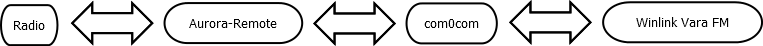
\includegraphics[width=0.8\textwidth]{../image/Diagram1.png}\\[0.4cm]
Normal inkoppling är att "Aurora-Remote" kopplas till radion och eventuellt ett komportspar till ett program som man vill använda radion till.
Komportspar kan skapas med hjälp av com0com.
\newline
\newline
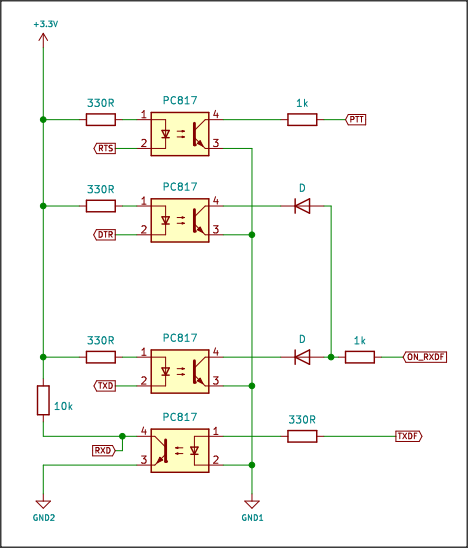
\includegraphics[width=0.5\textwidth]{../image/Interface.png}\\[0.1cm] 
En USB-TTL, exempelvis cp2102 eller ft232rl, kopplas till ovan schema.
\newline
Kontrollera vilken spänningsnivå som det är på RTS, DTR, m.m. så du väljer samma för drivningen av optokopplarna.

\newpage
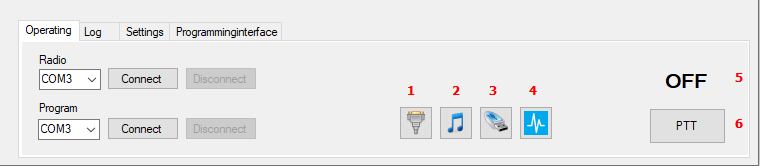
\includegraphics[width=0.5\textwidth]{../image/AuroraRemoteOperating.png}

\begin{enumerate}   
\item Genväg till com0com
\item Genväg till ljudinställningarna
\item Genväg till datorns systeminställningar
\item Genväg till datorns aktivitetshanterare
\item Status på meddelande och radion
\item Lyser rött när PTT aktiveras av ett program. Tryck på den för att aktivera PTT.
\end{enumerate} 

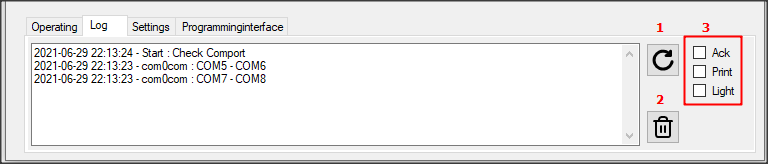
\includegraphics[width=0.5\textwidth]{../image/AuroraRemoteLog.png}
\begin{enumerate}   
\item Uppdaterar komportar
\item Tömmer loggrutan
\item Väljer vad som skall visas i loggen
\end{enumerate}  

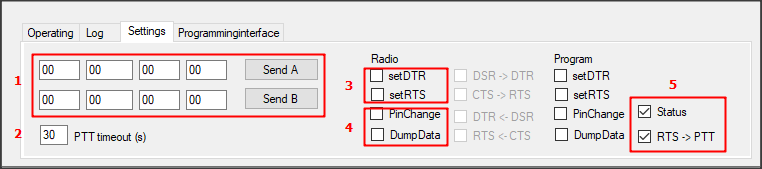
\includegraphics[width=0.5\textwidth]{../image/AuroraRemoteSettings.png}
\begin{enumerate}   
\item För att skicka kommando till radion
\item Maximala tiden för PTT
\item För att testa interfacet
\item Extra loggning
\item Stänger av funktioner för att kunna skicka meddelande till radion utan att automatiska meddelande stör. 
\end{enumerate}  

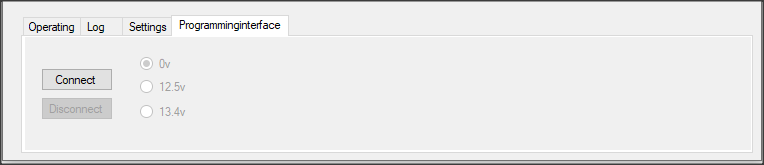
\includegraphics[width=0.5\textwidth]{../image/AuroraRemoteProg.png}
\begin{enumerate}   
\item Testar programmeringsinterfacet på   0.0v
\item Testar programmeringsinterfacet på 12.5v
\item Testar programmeringsinterfacet på 13.4v
\end{enumerate}  

\newpage


%% Section  Useful Links
\section*{Useful Links}

* Null-modem emulator (com0com) \href{https://sourceforge.net/projects/com0com/}{https://sourceforge.net/projects/com0com/}. 

%% Section License
\section*{License}

GNU General Public License v3.0


\end{document}